\documentclass{letter}

\usepackage[a4paper]{geometry} 
\usepackage{graphicx}
\usepackage{xcolor}

\begin{document}

\begin{center} \large\textbf{FOSSEE} \end{center}

\textbf{Free and Open Source Software in Education} ({\color{blue}http://fossee.in}) provides
free support on FOSS (free and open source software) to eliminate the use of
proprietary/commercial software packages in Science and Engineering Education
across India. The shift to FOSS packages will help educational institutions
monetarily. 

\vskip3ex

The flagship activities promoted by the FOSSEE team are:

\vskip3ex

%first column
\begin{minipage}[t]{0.48\linewidth} 
\textbf{Textbook Companion}: involves creating codes for solved examples of standard
textbooks using FOSS. It is available online for free download and use. The
contributors of these Textbook Companions are students and the faculty of colleges from different parts of
India. Students and faculty involved in Textbook Companion are given
 honorarium and certificates for their efforts.  
\end{minipage} \hspace{0.04\linewidth}
%second column
\begin{minipage}[t]{0.48\linewidth} 
\textbf{Lab Migration}: As long as a college uses proprietary tools as part of their lab
curriculum, we cannot eliminate the use of commercial software. The Lab
Migration activity aims to migrate college labs using proprietary software to a
FOSS only lab. The FOSS code created by a student/teacher is released in open
source code for public use. Students and faculty involved in Lab Migration are given
 honorarium.
\end{minipage}

\vskip5ex

%first column
\begin{minipage}[t]{0.48\linewidth} 
\begin{center}
    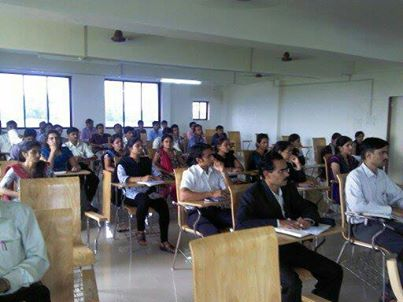
\includegraphics[width=1\linewidth]{images/self_workshops.jpg} 
    \textit{\small Photo: Spoken Tutorial SELF Workshop.}
\end{center}
\vskip3ex
\textbf{SELF Workshops \& Forum Support}: FOSSEE team provides domain expertise to 
SELF workshop(s) which are conducted by the Spoken Tutorial project.  
Additionally, the FOSSEE team provides forum support, ({\color{blue}http://forums.spoken-tutorial.org/}) 
where the students post queries if any, post-workshop. The FOSSEE domain experts duly answer these queries. 
\end{minipage} \hspace{0.04\linewidth}
%second column
\begin{minipage}[t]{0.48\linewidth} 
\begin{center}
    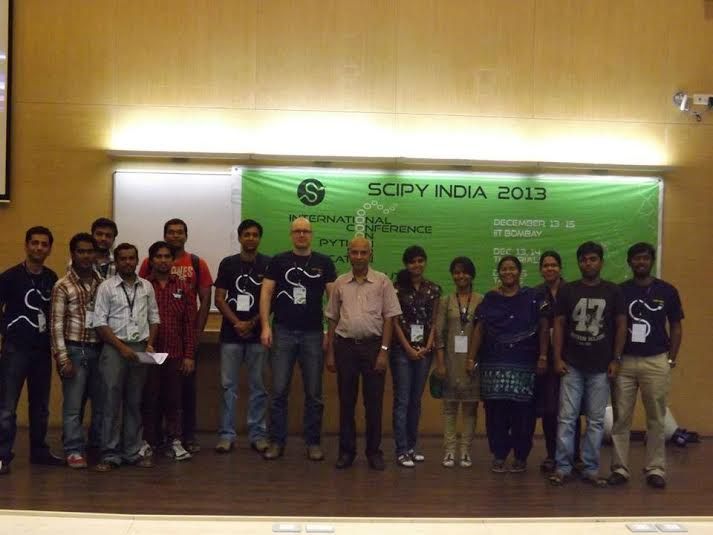
\includegraphics[width=1\linewidth]{images/scipy_2013.jpg} 
    \textit{\small Photo: 5th Scipy India Conference.}
\end{center}
\vskip3ex
\textbf{Conference}: Scipy India - an international conference on scientific computing
with Python, is organized every year by FOSSEE since 2009. One of the goals of
the conference is to combine education, engineering, and science with computing
through the medium of Python.  
\end{minipage}

\newpage 
Currently, FOSSEE team promotes the following software extensively: \\

% first column
\begin{minipage}[t]{0.48\linewidth} \begin{center}

\includegraphics[width=0.7\linewidth]{images/scilab_logo.png} \end{center}
\textbf{Scilab} is a free and open source software for numerical computation
developed by Scilab Enterprises, France. It is a FOSS alternative to MATLAB.
It also includes Xcos which is an open source alternative to Simulink. The
Scilab team have successfully created more than 275 Textbook Companions and
ported 12 labs through the Lab Migration activity till date. To increase ease
of executing Textbook Companion code online, FOSSEE has ported TBC on GARUDA
cloud {\color{blue}http://scilab.in/scilab-on-cloud}. Please visit {\color{blue}http://scilab.in} for
more details.  \end{minipage} \hspace{0.04\linewidth}
%second column
\begin{minipage}[t]{0.48\linewidth} \begin{center}
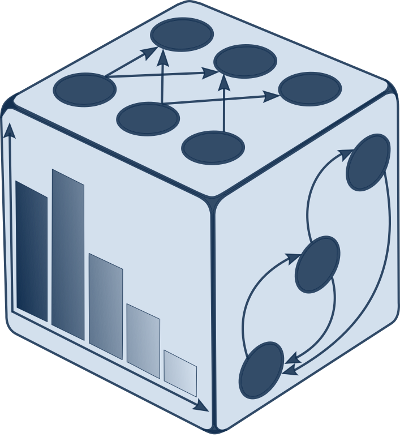
\includegraphics[width=0.25\linewidth]{images/coin_logo.png} \end{center}
\textbf{COIN-OR} or \textbf{CO}mputational \textbf{IN}frastructure for
\textbf{O}perations \textbf{R}esearch is a project to build and support an
open-source software for operations research and its applications.
\textbf{Simpy} (Simulation in Python) is an open source, Python-based,
discrete-event simulation software. OR Tools at FOSSEE is promoting COIN-OR,
Simpy and other FOSS by developing tutorials, textbook companions and software
interfaces in Scilab and Python. For more details please visit
{\color{blue}http://or.fossee.in} \end{minipage}

% first column
\begin{minipage}[t]{0.48\linewidth} \begin{center}

\includegraphics[width=0.32\linewidth]{images/cfd_logo.png} \end{center}
\textbf{OpenFOAM} is a free, open source CFD software package developed by
OpenCFD Ltd and distributed by the OpenFOAM Foundation. Tutorials in the form
of web-casts, for self learning OpenFOAM have been developed by our team. These
are available free of cost at {\color{blue}http://cfd.fossee.in}.  \end{minipage}
\hspace{0.04\linewidth}
%second column
\begin{minipage}[t]{0.48\linewidth} \begin{center}

\includegraphics[width=0.32\linewidth]{images/python_logo.png} \end{center}
\textbf{Python} is a general-purpose interpreted, high-level, object-oriented
programming language that is used in a wide variety of application domains.The
Python team promotes the use of the language through Python Textbook Companion.
Under Python Textbook Companion, 53 textbook companions have been completed.
For more information visit {\color{blue}http://python.fossee.in/} \end{minipage}

\begin{minipage}[t]{0.48\linewidth} \begin{center}

\includegraphics[width=0.32\linewidth]{images/oscad_logo.png} \end{center}
\textbf{Oscad} is developed by the FOSSEE team at IIT Bombay. It is an EDA tool
for circuit design, simulation, analysis and PCB design. Free tutorials of
Oscad are available at {\color{blue}http://oscad.in/resources/tutorials}.  \end{minipage}

\end{document}
